%Tim Dixon
%%Main takeaway - we provide calving front locations, and have automated it
%Some may be more interested in the data, or the method, so make sure we cover both

\documentclass[tc,manuscript]{copernicus}

\usepackage{wrapfig}
\usepackage{booktabs}
\usepackage{colortbl}
\usepackage{pdflscape}
\begin{document}

\title{Supplement of Calving Front Machine (CALFIN): Automated Calving Front Dataset and Deep Learning Methodology for East/West Greenland, 1972-2019}

\Author[1]{Daniel}{Cheng}
\Author[1]{Yara}{Mohajerani}
\Author[2]{Michael}{Wood}
\Author[2]{Eric}{Larour}
\Author[1]{Wayne}{Hayes}
\Author[1]{Isabella}{Velicogna}
\Author[1,2]{Eric}{Rignot}


\affil[1]{University of California at Irvine, Irvine CA, USA}
\affil[2]{Jet Propulsion Laboratory, California Institute of Technology, Pasadena CA, USA}

\runningtitle{TEXT}

\runningauthor{TEXT}

\correspondence{Daniel Cheng (dlcheng@uci.edu)}

\received{}
\pubdiscuss{} %% only important for two-stage journals
\revised{}
\accepted{}
\published{}

\maketitle


%\tableofcontents

\section{Dataset}
\subsection{Usage}
(Petermann example)
(NSIDC writeup)
\subsection{Shapefile Metadata}
(NSIDC writeup)


\begin{landscape}
    \subsection{Temporal Availability}
    \begin{figure}[h]
        \centering
        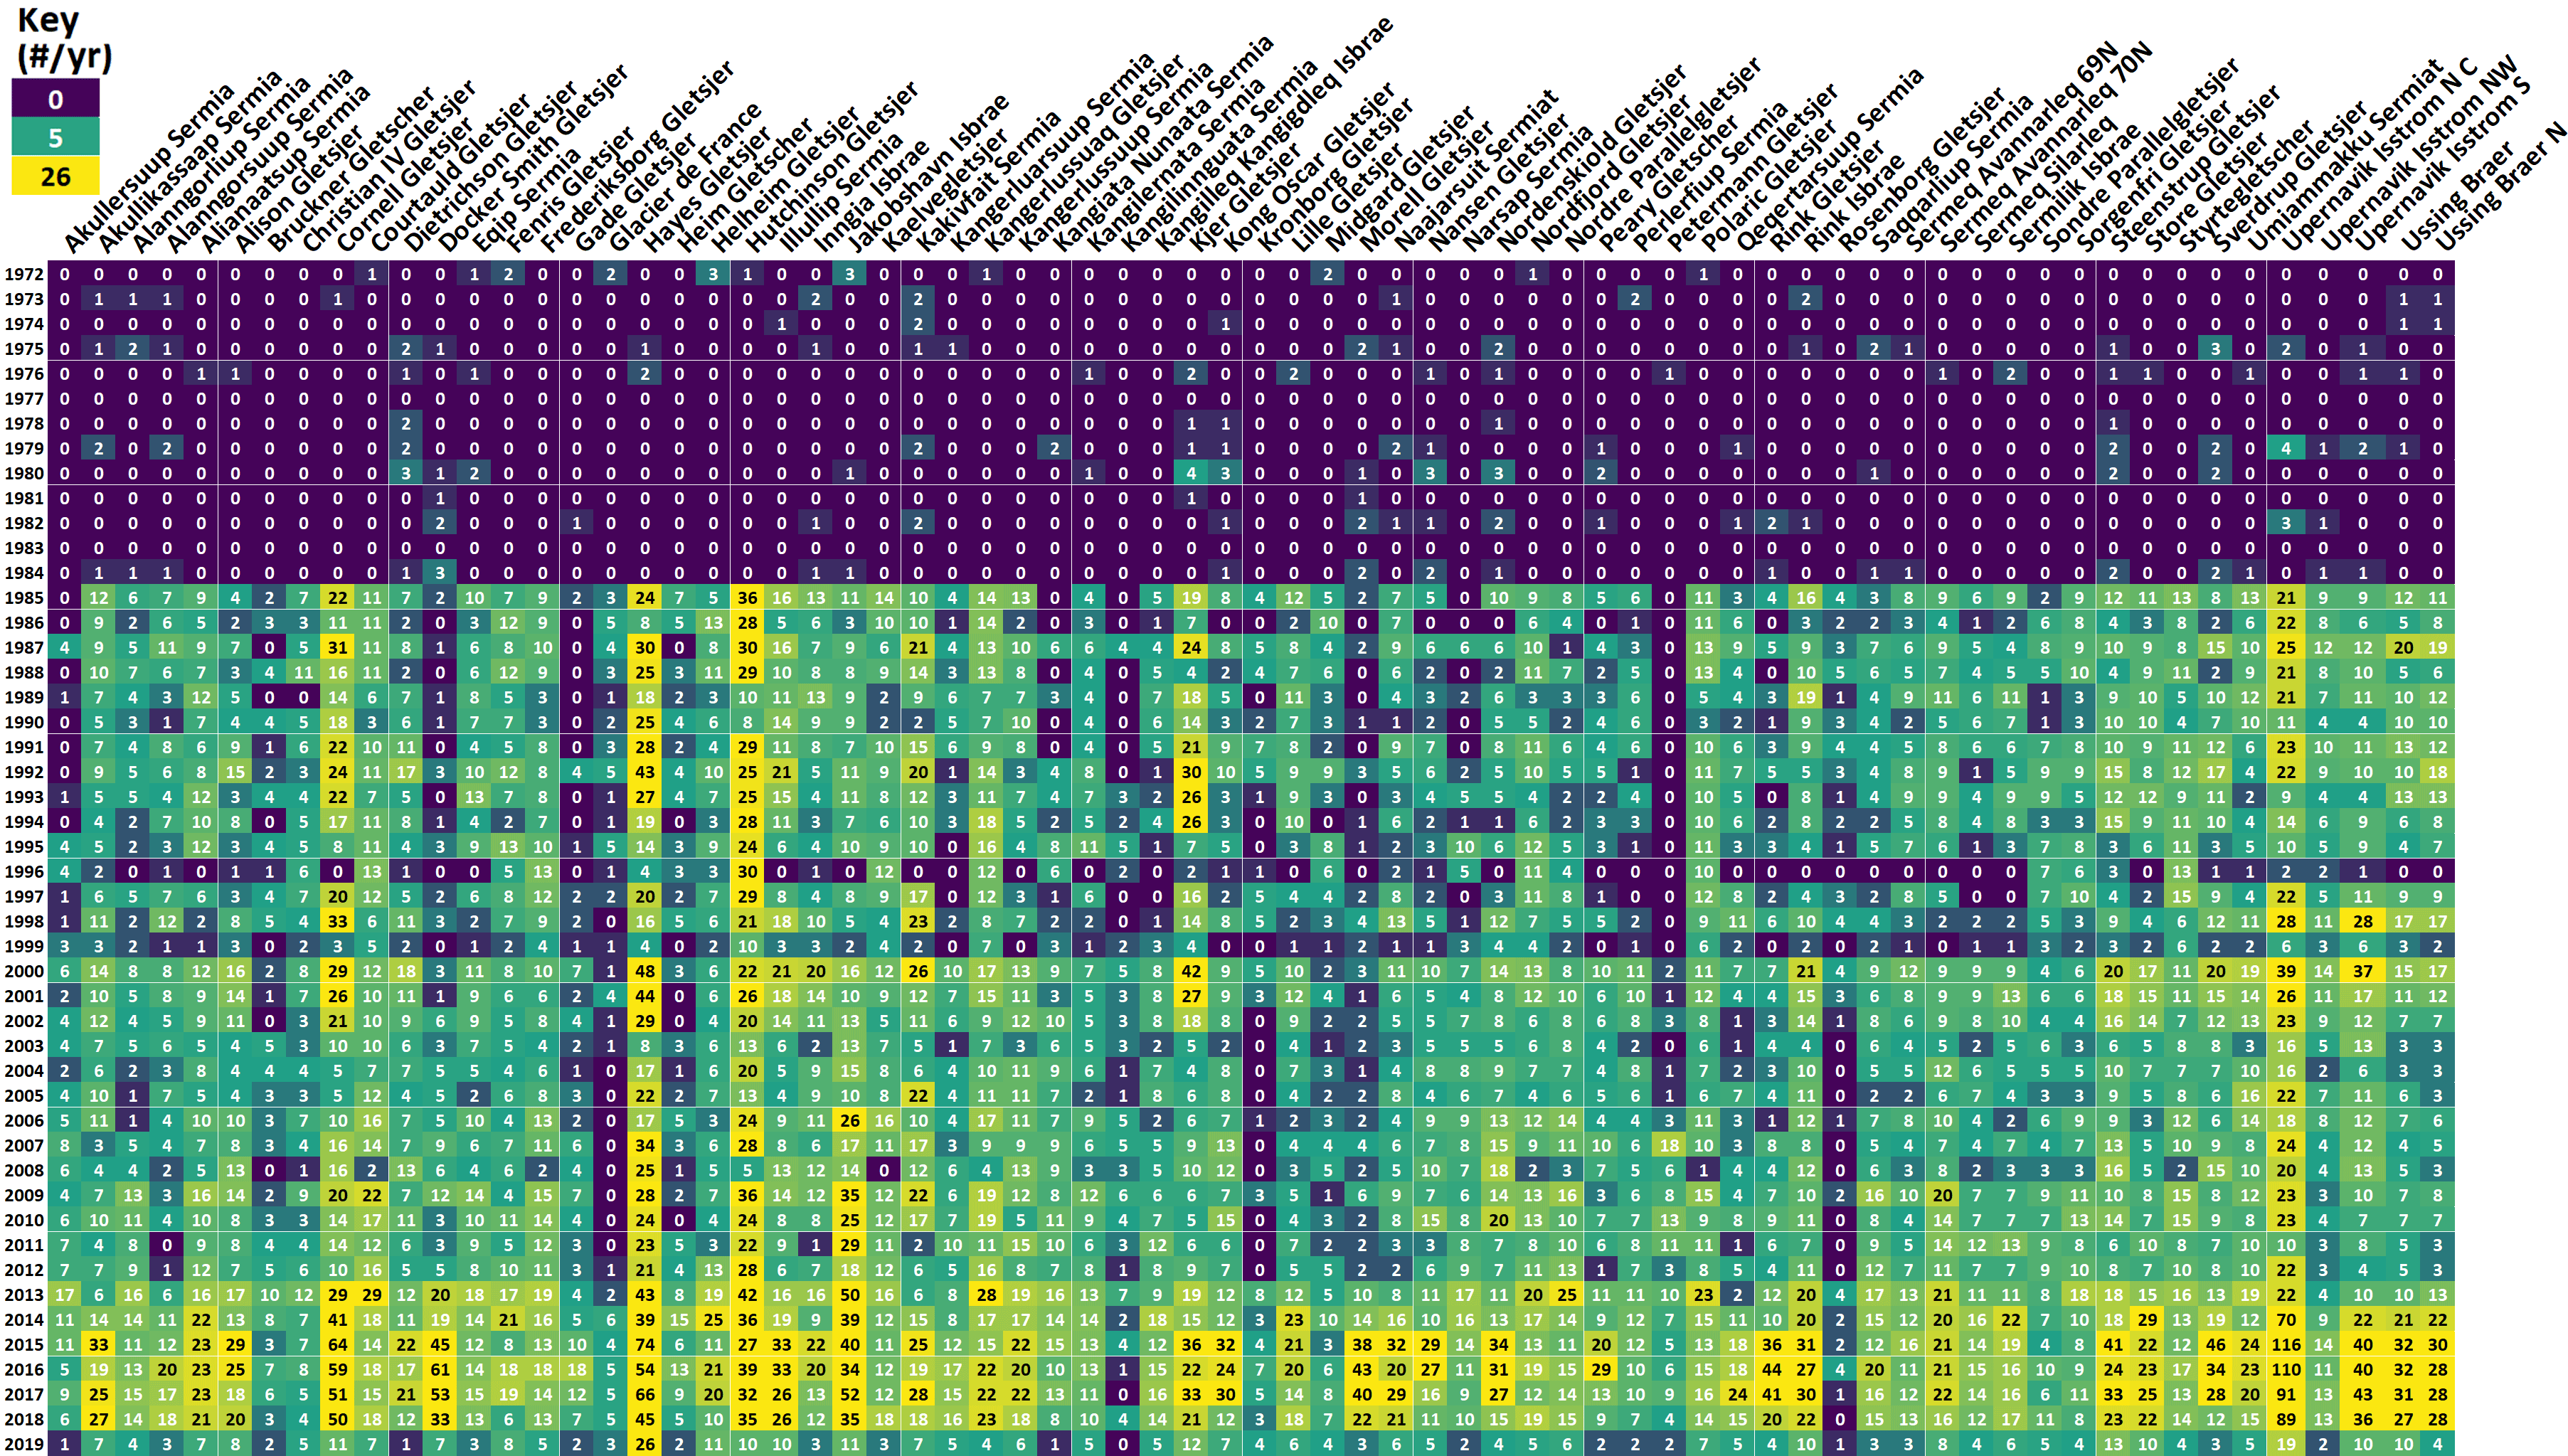
\includegraphics[width=21cm]{figures/temporal_all.png}
        \caption{Number of images per year for all 67 glaciers in the CALFIN dataset.}
        \label{fig:temporal_all}
    \end{figure}
\end{landscape}


%full pipeline
\section{Training Data}
(Image grid)

\section{Inter-model Comparison Table}

% \usepackage{booktabs}
% \usepackage{colortbl}

% \usepackage{booktabs}
% \usepackage{colortbl}


\begin{table}[h]
\centering
\setlength{\extrarowheight}{0pt}
\addtolength{\extrarowheight}{\aboverulesep}
\addtolength{\extrarowheight}{\belowrulesep}
\setlength{\aboverulesep}{0pt}
\setlength{\belowrulesep}{0pt}
\begin{tabular}{cccccc} 
\toprule
\rowcolor[rgb]{0.71,0.71,0.71} Validation Set & Model & Mean Distance & Median Distance & IoU Coastline & IoU~Ice/Ocean \\ 
\hline\hline
CALFIN-L7SCE-none & CALFIN & 2.27px, 81.65m & 1.16px, 44.01m & 0.4880 & 0.9819 \\
\rowcolor[rgb]{0.886,0.886,0.886} CALFIN-L7SCE-only & CALFIN & 2.22px, 91.93m & 1.33px, 49.24m & 0.4888 & 0.9766 \\
\hline
CALFIN & CALFIN & 2.25px, 86.76m & 1.21px, 44.59m & 0.4884 & 0.9793 \\
\rowcolor[rgb]{0.886,0.886,0.886} CALFIN & Mohajerani & 4.45px, 201.35m & 1.25px, 50.52m & 0.4935 & 0.9699 \\ 
\hline
Mohajerani & CALFIN & 2.56px, 97.72m & 2.55px, 97.44m & 0.3332 & N/A \\
\rowcolor[rgb]{0.886,0.886,0.886} Mohajerani & Mohajerani & 1.97px, 96.31m & N/A & N/A & N/A \\ 
\hline
Zhang & CALFIN & 3.56px, 284.22m & 1.69px, 114.50m & 0.3739 & 0.9778 \\
\rowcolor[rgb]{0.886,0.886,0.886} Zhang & Zhang & 17.3px, 104m & N/A & N/A & N/A \\ 
\hline
Baumhoer & CALFIN & 3.36px,543.47m & 0.95px,127.87m & 0.5959 & 0.9873 \\
\rowcolor[rgb]{0.886,0.886,0.886} Baumhoer & Baumhoer & 2.69px, 108m & N/A & N/A & 0.905 \\
\bottomrule
\end{tabular}
\end{table}



\begin{landscape}
    \section{Quality Assurance \& Validation}
    \subsection{Quality Assurance}
    \begin{figure}[h]
        \centering
        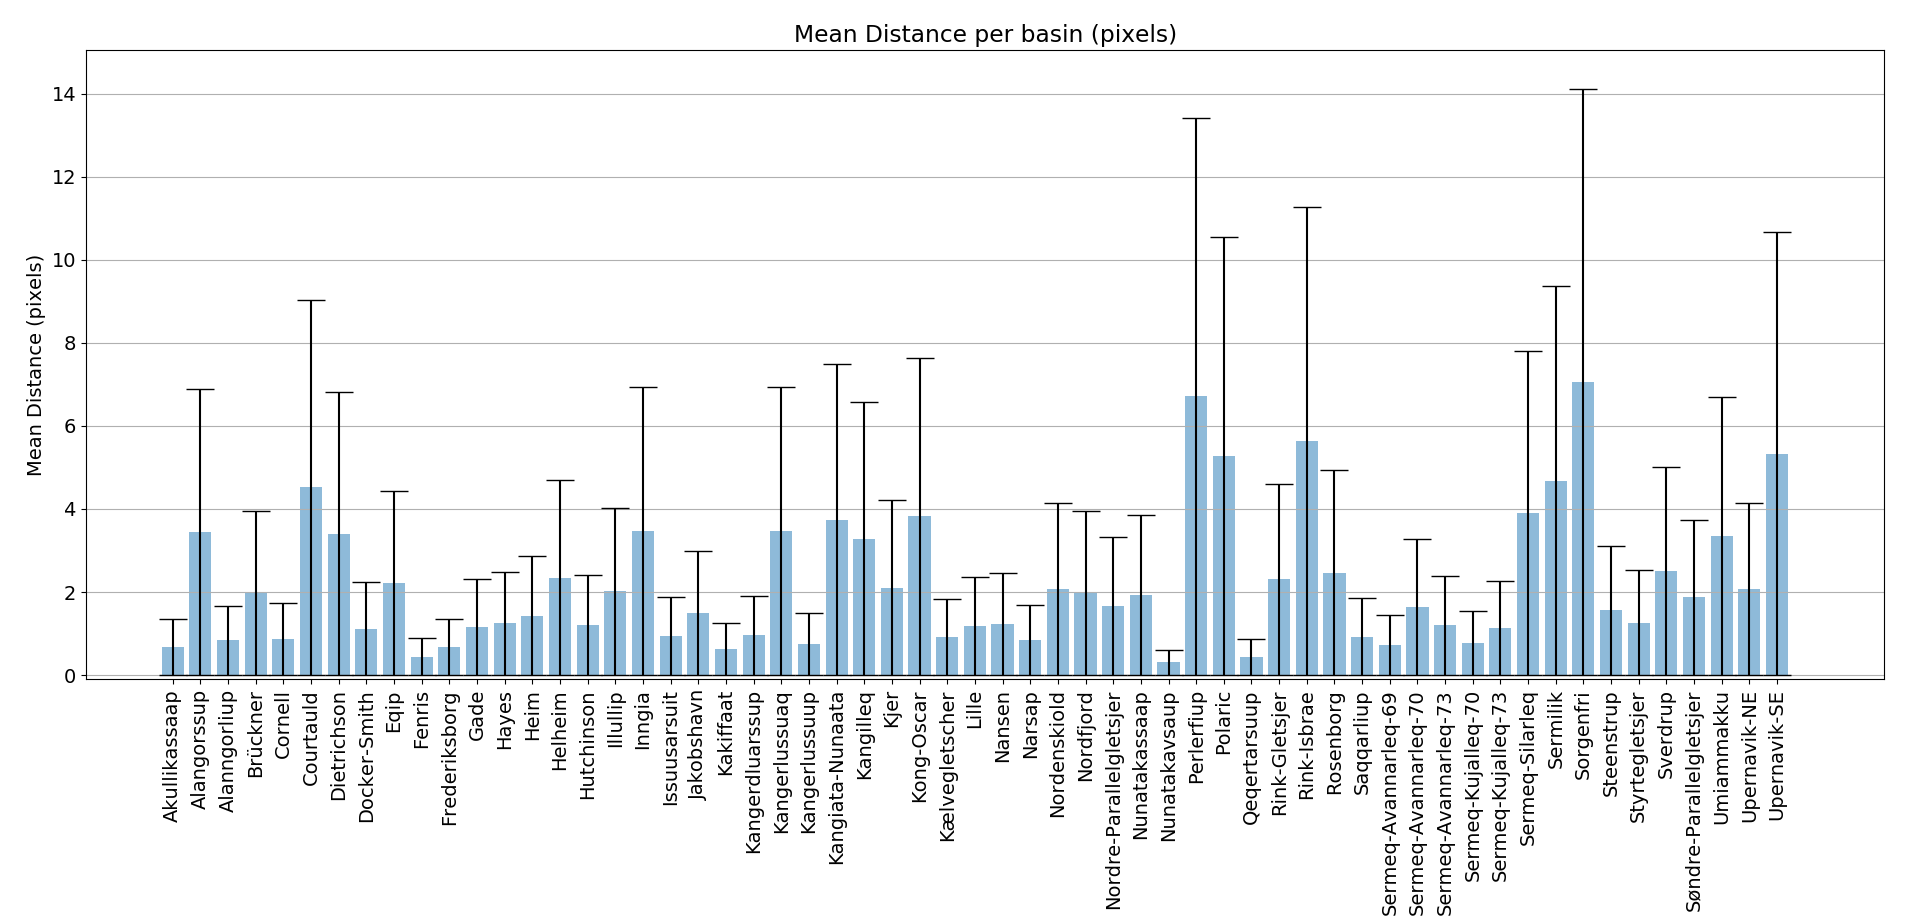
\includegraphics[width=21cm]{figures/mean_distancce_basin_pixels.png}
        \caption{True mean distance error estimates per basin, in pixels.}
        \label{fig:temporal_all}
    \end{figure}
\end{landscape}

\subsection{CALFIN Validation Set}
\subsection{Mohajerani et al. Validation Set}
\subsection{Zhang et al. Validation Set}
\subsection{Baumhoer et al. Validation Set}
\end{document}